\documentclass{minimal}
\usepackage{tikz}
\usetikzlibrary{arrows}
\begin{document}
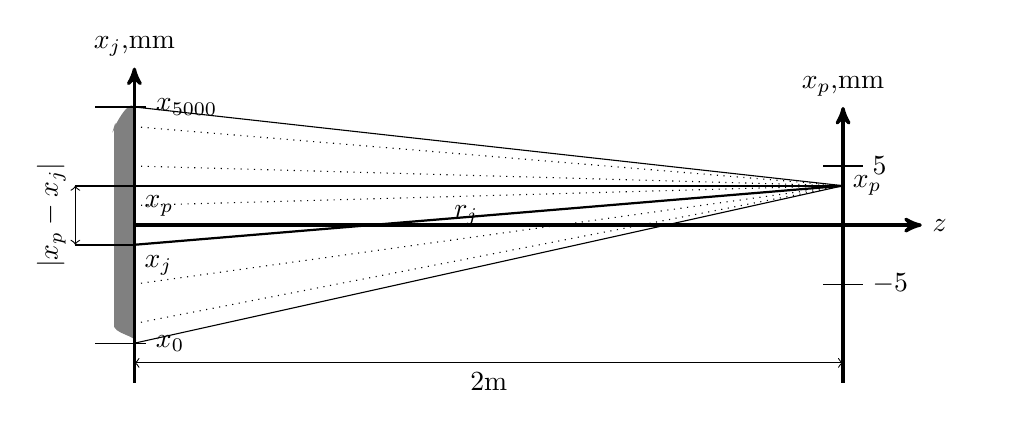
\begin{tikzpicture}[
    scale=5,
    axis/.style={very thick, ->, >=stealth'},
    important line/.style={thick},
    dashed line/.style={dashed, thin},
    pile/.style={thick, ->, >=stealth', shorten <=2pt, shorten
    >=2pt},
    every node/.style={color=black}
    ]
    % axis
    \draw [gray, fill=gray] (-0.05,0.15) -- (-0.05, 0.65)  to[out=250] (0,0.7)
    -- (0,.1) to[in=250] (-0.05,0.15);
 
    \draw[axis] (0,0.4)  -- (2,0.4) node(xline)[right]  {$z$};
    \draw[axis] (0,0) -- (0,0.8) node(yline)[above] {$x_j$,mm};
     \draw[axis] (1.8,0.0) -- (1.8,0.7) node(yline)[above] {$x_p$,mm};

    % Lines
    \draw[dotted] (0,.45) coordinate (A) -- (1.8,.5)
        coordinate (B) node[right, text width=5em] {$x_p$};
	\draw[important line] (0,.35)node(xline)[below right]{$x_j$}  --(0.9,0.425)node(yline)[left]{$r_j$}-- (1.8,.5);
	\draw[important line] (0,.5) node(xline)[below right]{$x_p$}-- (1.8,.5);
	\draw[important line] (-.15, .5) --(0,.5);
	\draw[important line] (-.15, .35) --(0,.35);
	\draw[<->] (-.15,.5) -- (-.15,.425)node(yline)[above,rotate=90]{$|x_p-x_j|$} -- (-.15,.35);
	\draw[dotted] (0,.25)  -- (1.8,.5);
	\draw[dotted] (0,.15) --(0.9, 0.325) node(yline)[below]{} -- (1.8,.5);
	\draw[dotted] (0,.55)  -- (1.8,.5);
	\draw[dotted] (0,.65)  -- (1.8,.5);
	\draw (0,.7)  -- (1.8,.5);
	\draw(0,0.1) --(1.8,.5);
	\draw (-0.1, 0.1) -- (0.03, 0.1) node(yline)[right] {$x_0$};
	\draw (-0.1, 0.7) -- (0.03, 0.7) node(yline)[right] {$x_{5000}$};
	\draw (1.75, 0.25) -- (1.85, 0.25) node(yline)[right] {$-5$};
	\draw (1.75, 0.55) -- (1.85, 0.55) node(yline)[right] {$5$};
	\draw[<->](0,0.05)--(0.9,0.05)node(yline)[below]{$2$m} --(1.8,0.05) ;
    
\end{tikzpicture}
\end{document}